\pagebreak
\section{Daten bekommen}
\label{getData}

Auf der Website werden wiederholt Daten vom Server geholt. Dies mache ich mit einem \textit{fetch}.
Mit dem Fetch Befehl und den richtigen API-Link konnte ich mur so immer die Daten holen, die ich
gebraucht habe. 


Im Projekt selbst habe ich einen Custom Fetch verwendet, welcher zusätzlich zu den Daten auch einen 
Error liefert, falls der Fetch fehlschlägt, als so wohl auch eine boolean Variable, welche true ist und 
erst false wird, wenn alle Daten vom Server an der Website angekommen ist. Diese Variable genannt 
\textit{isPending} ist in dem Sinne von nützen, dass der Nutzer informiert wird, dass die Daten noch
laden müssen.

\begin{lstlisting}
import { useState, useEffect } from 'react';
import Error from '../staticViews/Error'

const useFetch = url => {
  const [data, setData] = useState(null);
  const [isPending, setIsPending] = useState(true);
  const [error, setError] = useState(null);

  useEffect(() => {
    const abortCont = new AbortController();

    setTimeout(() => {
      fetch(url, {
        method: 'GET',
        signal: abortCont.signal })
        .then(res => {
          if (!res.ok) {
            throw Error('Daten konnten nicht empfangen werden');
          }
          return res.json();
        })
        .then(data => {
          setIsPending(false);
          setData(data);
          setError(null);
        })
        .catch(err => {
          if (err.name === 'AbortError') {
            console.log('fetch abgebrochen')
          } else {
            setIsPending(false);
            setError(<Error></Error>);
          }
        });
    });

    return () => abortCont.abort();
  }, [url]);

  return { data, isPending, error };
};

export default useFetch;

\end{lstlisting}

Wie man im Code sehen kann, werden die drei Variablen mit einem \textit{setState} und dem Wert null
deklariert. Außer \textit{isPending} welche wie oben schon genannt standardmäßig auf true ist. Diese
drei Werte werden am Ende als return Wert zurückgegeben um sie dann außerhalb des useFetch benutzen 
zu können.


Falls ein Fehler auftritt, wird der State der Error Variable auf eine Error Komponente gesetzt. Dies
habe ich gemacht um bei jedem Fetch dem Benutzer eine Einheitliche Fehlermeldung zu geben, falls ein 
Fehler auftritt.


Diese Fehlermeldung sieht wie folgt aus:
\begin{figure}[H]
    \begin{center}
      \frame{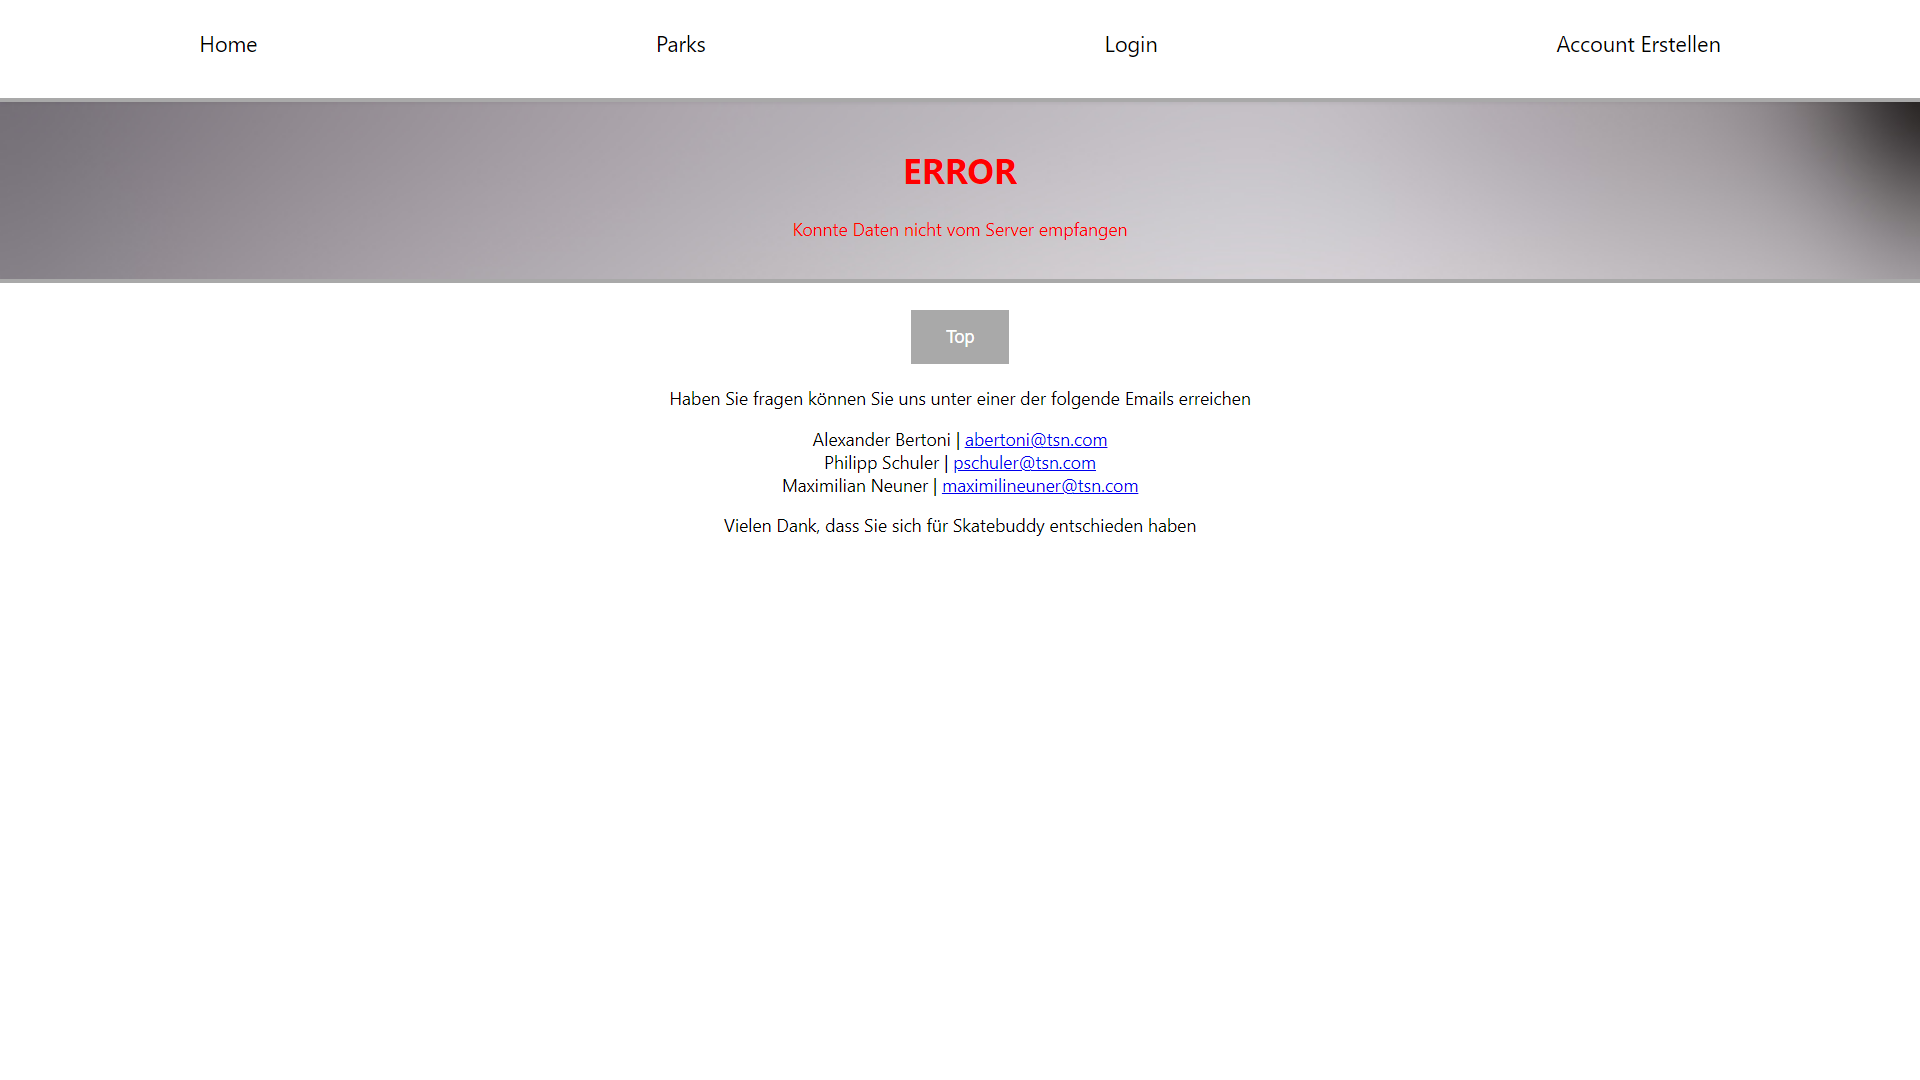
\includegraphics[width=1\textwidth]{Website/ErrorMessage.png}}
      \caption{Fehlermeldung wenn das Daten holen vom Server fehlschlägt}
    \end{center}
  \end{figure}
  